\documentclass[UTF8]{ctexart}

%opening
\title{审稿意见的回复}
\author{周勇}

\begin{document}

\maketitle

本文的目标是验证PSD的大动态范围读出设计能够覆盖直到Z=20的相对论论能区的重离子信号。
为了消除误解,首先对文章中大动态范围的验证过程进行一个梳理。
\begin{enumerate}
  \item 实验得到了Z=2-8的中能重离子的单元条中心响应结果。
  \item 利用能损和光输出的线性关系,推出Z=2-8的相对论重离子的单元条中心响应结果。
  \item 利用BTV模型,基于Z=2-8的相对论重离子的单元条中心响应结果外推到Z=20。
  \item 利用实验得到的衰减长度,得到单元条端头信号相对于中心信号的倍数。
  \item 综合入射角度,能量涨落以及光传输衰减,估算出PSD的最大信号大小。
  \item 最大信号的幅度在PSD读出电子学的线性范围内,从而验证了PSD的大动态范围读出设计的合理性。
\end{enumerate}

\section{意见(1)}
问:文中只进行了轻带电粒子的实验验证,而探测器的电子,伽玛探测性能等并未进行测量和分析,建议作者缩小文章中文题目的范围。

答:
在DAMPE的目标能区范围内,入射粒子都处于相对论能区,它们在在PSD单元条的能量损失有以下几个特点:
\begin{enumerate}
 \item 高能光子在PSD中没有能量沉积。
 \item 高能电子在PSD中的沉积能量来自电离能损,其大小约为1MIPs。
 \item 高能重离子在PSD中的沉积能量来自电离能损,其大小正比于$Z^2$。而且,对于相同种类的重离子,其在PSD中的能损与速度关联不大(处于相对论坪区)。
\end{enumerate}
由于$\gamma$在PSD中没有沉积能量,它对动态范围大小没有贡献;而电子的沉积能量与Z=1的重离子是差不多的,约为1MIP,它对动态范围的贡献与Z=1的重离子是一致的。
而不同种类重离子的能损差别巨大,PSD动态范围的大小最终由重离子决定。
正如文章标题所示,本文的重心是大动态范围的实验验证,并不是PSD探测单元模块的性能测试,因此不需要涉及电子和伽玛探测性能的讨论。

\section{意见(2)}
问:有关探测器灵敏面积的数据820mm x 820mm,单元条长度为884mm x 28mm X 10mm,按照82个排列,应该是以10mm长度作为灵敏面,而28mm作为探测器的厚度面,但是文中及计算均采用了10mm作为厚度计算,另外884mm的长度没有完全计算在PSD的灵敏面积内,请解释。

答:PSD实际由两个相互垂直的探测平面组成,见图~\ref{fig:psd}。两个探测平面构型完全一样,但单元条方向相互垂直。每个探测由41个探测单云模块紧密排列组成,且相邻单元有重叠部分。
这是为了消除单元间的间隙,消除探测器死区。单元条宽度为28mm,厚度为10mm,由于重叠部分的存在,最后的有效探测面积为$820mm\times820mm$。
原文中的文字较简略,容易引起误解,认为PSD只有一个探测平面,修改稿中增加了这部分的描述。

\begin{figure}[htp]
 \centering
 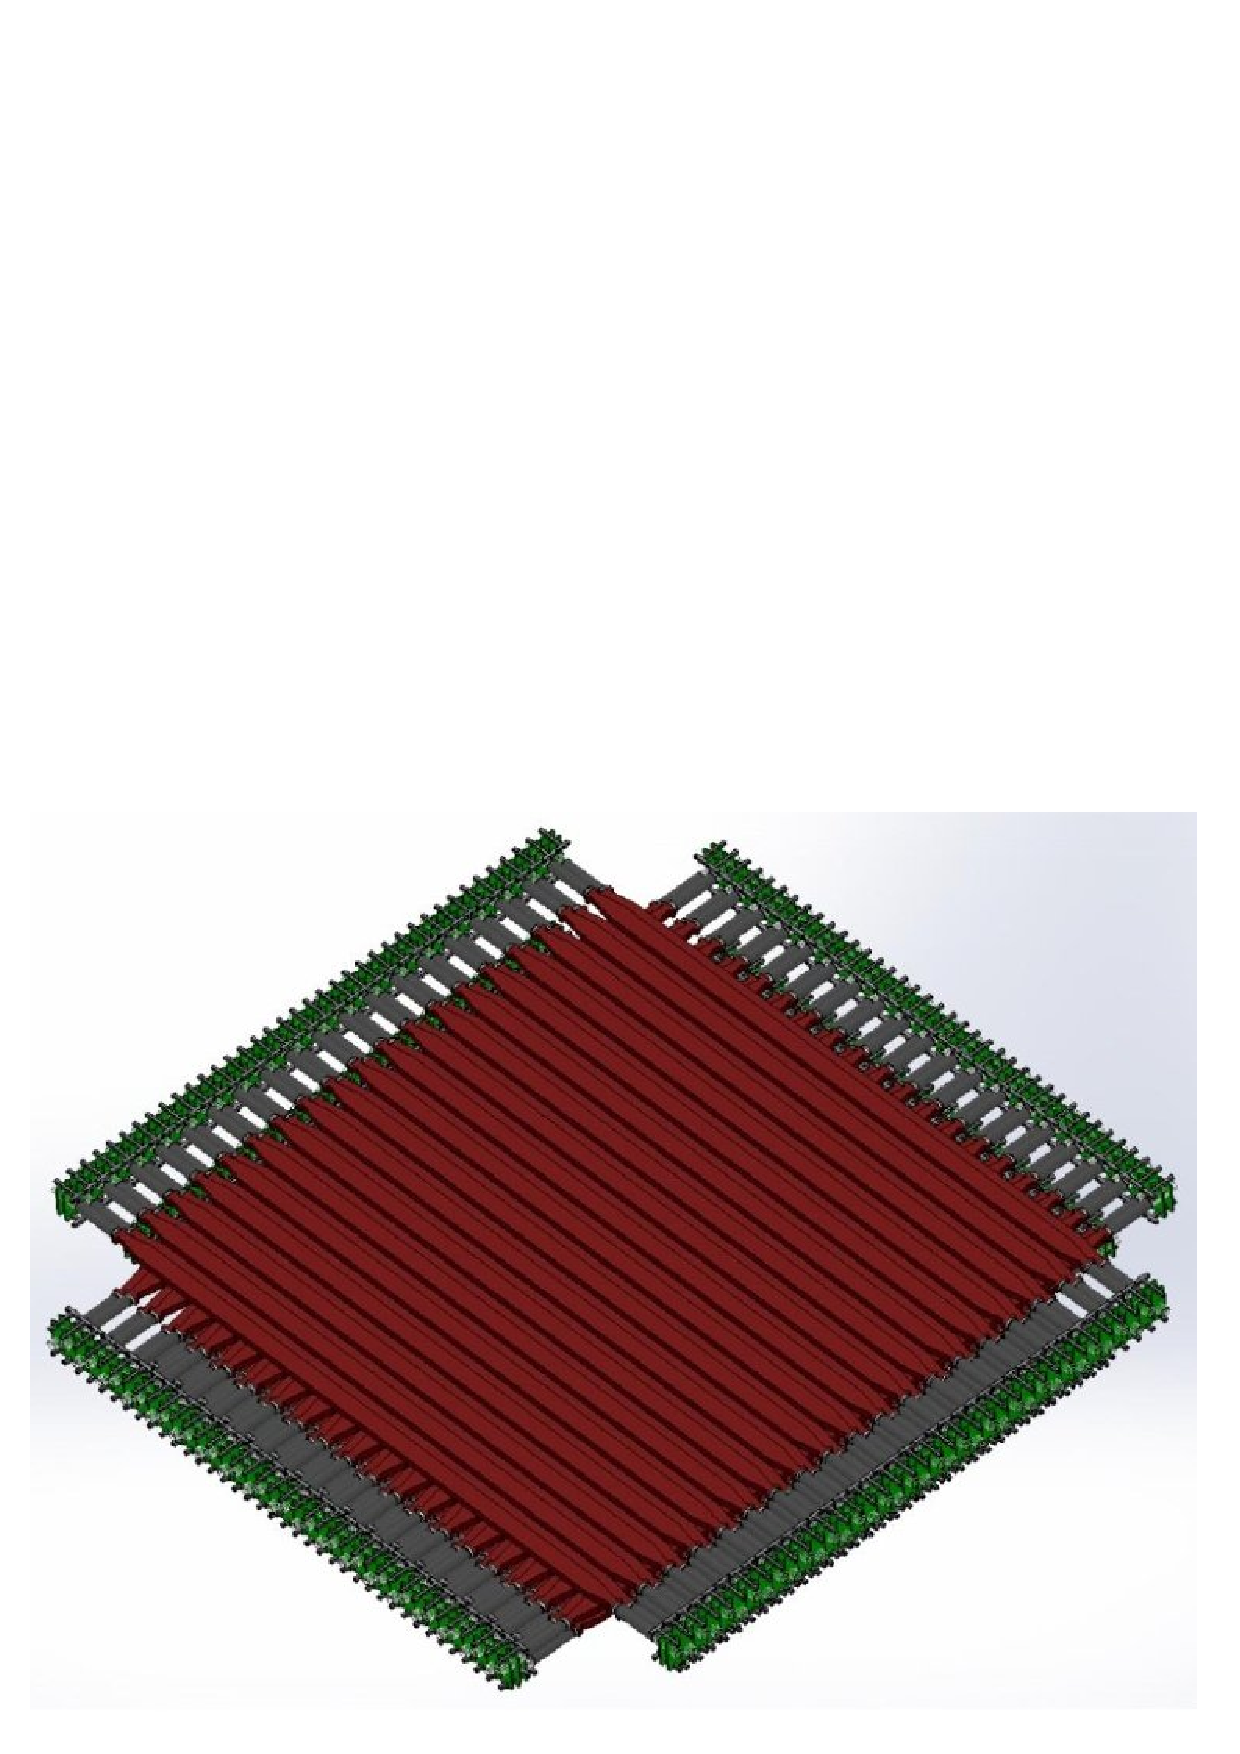
\includegraphics[width=0.8\textwidth]{psd.jpg}
 \caption{PSD构型}
 \label{fig:psd}
\end{figure}

\section{意见(3)}
问:图2及文中描述采用了不同能量的16O束流进行了测试,且图2中并未出现16O主束,和3He鉴别,而图3的投影图中有16O和3He,请作者检查并解释。

答:分三个方面讨论:
\begin{enumerate}
   \item 实验中用了三种束流配置,这在文章中有介绍。每种配置条件下,都对应一个的TOF-$\Delta$E图。由于是三种不同的实验条件,所以它们不能也不适合在同一副图中展示。
   图2是其中一个束流配置下的结果,此条件下次级核素最多,也是实验中测试时间最长的束流配置。
   \item 另外,图2主要作为一个示例在文章使用,它展示本次实验如何对次级核素进行鉴别,是对实验条件的描述。其它两种配置条件下有类似的结果。
   \item 图3和图2并不完全对应。图3是实验结果的展示,因此它整合了所有测试数据,包括了三种配置条件下的所有测试结果。而图2是实验条件的展示,它只对应其中一个束流配置条件。
  \end{enumerate}


\section{意见(4)}
问:表1上方,能量响应中心值L和能损的关系是如何推得的,请解释。

答:这在原文第三节的一二两段有详细的描述,修改稿中对容易引起误解的地方进行了补充。
本次实验能够直接得到的是PSD单元条对中能重离子束的响应(即L),而我们希望得到的是单元条对相对论能区重离子的响应(为了消除误解,修改稿中用$L_{mip}$明确表示这个量)。
使用LISE还可以计算出实验中所用的中能重离子在单元条中的能损$\Delta E_{exp}$和对应的相对论能区重离子在单元条的能损$\Delta E_{mip}$。
因此,这个问题就演变成从已知量$L$、$\Delta E_{mip}$和$\Delta E_{exp}$推出未知量$L_{mip}$。
其根据就是“对于同一种重离子来说,在沉积能量相差不大的条件下,其在塑闪中的光产额近似与沉积能量大小成正比”,从而得到
\begin{equation}
L_{mip}=L\frac{\Delta E_{mip}}{\Delta E_{exp}}
\label{eq:correction}
\end{equation}
即修改稿中的公式(1)

\section{意见(5)}
问:图4上方文字“其中横轴为电荷数Z”,对比图4应该为$Z^2$。图4中Dy5对应的道数和图3道数不符,例如16O在图3中为1700chn左右,这样外推出来的Z=20的道数就可能会超出范围了,请解释。

答:原文中“其中横轴为电荷数Z”是笔误,修改稿中已经改为“其中横轴为电荷数$Z^2$”。
图3和表1分别是本次实验得到的原始谱和对应的拟合结果,是单元条的中能重离子响应。
而最终的动态范围验证是相对于相对论能区重离子的,从轻核到重核的外推也是基于相对论重离子。
因此,图4中的纵轴是相对论能区重离子在PSD单元条中的dy5通道响应中心值(即$L_{mip}$),其数值是将表1中的实验结果带入到公式(1)计算得到的。
以$^{16}O$为例,根据表1中的数值,可以计算得到它对应的相对论能区响应中心值为$1718.5*131.0/255.6=880.8$,结果与图4中一致。
为了消除误解,修正稿中明确了对图4纵轴的描述,图4中纵轴的题名也改为了$L_{mip}$。

\section{意见(6)}
问:引用文献2还未发表?建议引用作者已经发表的一些相关文献。

答:该文献已上传到arxiv(http://arxiv.org/abs/1601.07234),修改稿中已改为arxiv号引用。

\end{document}
